\chapter{Технологическая часть}
\section{Выбор и обоснование языка программирования и среды разработки}
При выборе языка программирования важно учитывать много факторов в 
зависимости от задачи. Из-за поставленной задачи на сцене будет несколько объектов, которые будут
перемещаться и изменяться, что будет создавать большую нагрузку на процессор.
В качестве языка программирования (ЯП) был выбран Си++. На это есть 
несколько причин:
\begin{enumerate}
    \item Данный язык программирования имеет большую производительность, что играет большую роль в выбранном алгоритме.
    \item Данная задача просто реализуется при использовании объектно-ориентированного подхода, который поддерживается данным языком.
    \item Используя стандартную библиотеку языка возможно создание всех требуемых структур данных, выбранных в результате проектирования.
\end{enumerate}
В качестве среды разработки был выбран CLion, так как:
\begin{enumerate}
    \item Использует утилиту CMake, что позволит конфигурировать проект независимо от платформы.
    \item Упрощает использование библиотек с помощью удобного интерфейса.
    \item Обладает необходимым функционалом для сборки, профилирования и отладки программ.
\end{enumerate}



\section{Реализация алгоритмов}
\begin{lstlisting}[label = lst:raytrace,caption= {Алгоритм обратной трассировки луча}]
    void Renderer::rayTrace(const Ray& tracedRay, ColorRGB& finalColor, std::shared_ptr<Scene> scene, int curDepth)
{
	std::shared_ptr<BaseShape> closestShape;
	float t = maxRange;
	for (auto shape : scene->getModels())
	{

		float intersection_t = shape->intersection(tracedRay);
		
		if (intersection_t > 0 || fabs(intersection_t) < EPS)
		{
			t = std::min(t, intersection_t);
			closestShape = std::dynamic_pointer_cast<BaseShape>(shape);
		}
	}
	if (fabs(t - maxRange) < EPS)
	{
        return;
    }
	std::shared_ptr<BaseLightSource> currentLightSource = scene->getLightSource();
	VecD3 intersectionPoint = tracedRay.getPoint(t);
	VecD3 lightVector = normalise(intersectionPoint - currentLightSource->getPosition());

	Ray lightRay(intersectionPoint,lightVector);
    
	if (hasIntersection(lightRay,scene))
		return;

	VecD3 shapeNormal = normalise(closestShape->getNormal(intersectionPoint));

	Material shapeMaterial = closestShape->getMaterial();
	float ambientIntensivity = shapeMaterial._k_a * currentLightSource->getIntensivity();
	finalColor = shapeMaterial._color * ambientIntensivity + finalColor;
	float diffuseLight = dot(shapeNormal, lightVector);
	if (shapeMaterial._k_d > 0)
	{
		if (diffuseLight > 0)
		{
			
			ColorRGB diffuseColorRay = currentLightSource->getColor() * diffuseLight * shapeMaterial._k_d;
			finalColor = shapeMaterial._color * diffuseColorRay + finalColor;

		}
	}
	if (shapeMaterial._k_s > 0)
	{

		Ray reflected = tracedRay.calculateReflected(shapeNormal, intersectionPoint);
		float specularDot = dot(reflected.D, tracedRay.D);
	
		if (specularDot > 0.0)
		{
			finalColor = currentLightSource->getColor() * specularDot * shapeMaterial._k_s + finalColor;
		}
	}
	if (shapeMaterial._k_s > 0.0f)
	{
		VecD3 N = closestShape->getNormal(intersectionPoint);
		Ray reflected = tracedRay.calculateReflected(shapeNormal, intersectionPoint);
		if (curDepth < maxDepth)
		{
			ColorRGB rcol(0, 0, 0);
			rayTrace(reflected, rcol, scene, curDepth + 1);
			finalColor = rcol * shapeMaterial._k_s * closestShape->getMaterial()._color + finalColor;
		}
	}
	float rayLength = (intersectionPoint - tracedRay.E).length();
	finalColor = finalColor / rayLength;
}
\end{lstlisting}

Заметим, что в листинге \ref{lst:raytrace} при трассировки луча сразу проверяется наличие пересечения с объектами сцены луча, исходящего к источнику света.
В данном случае tracedRay обозначает анализируемый в данный момент луч, finalColor - финальный цвет пикселя, scene - вектор указателей на примитивы, curDepth - текущая эпоха луча.


\begin{lstlisting}[label = lst:sphere_intersection,caption= {Алгоритм поиска пересечения со сферой}]
    double Sphere::intersection(const Ray& ray)
    {
        VecD3 origin  = ray.E - this->_center;
        float a = dot(ray.D, ray.D);
        float b = 2.0f * dot(origin, ray.D);
        float c = dot(origin, origin) - _radius * _radius;
        float discriminant = b * b - 4 * a * c;
        if (discriminant < 0)
            return -1.0; 
        else
        {
            float discriminant_value = sqrt(discriminant);
            double t1 = (-b + discriminant_value) / (2 * a);
            double t2 = (-b - discriminant_value) / (2 * a);
            if (t1 < 0 && t2 < 0)
                return -1.0;
            float t = std::min(t1, t2);
            if (t < 0)
            {
                if (t1 < 0)
                    t = t2;
                else if (t2 < 0)
                    t = t1;
            }
            return t;
        }
    
    }
\end{lstlisting}

Алгоритм \ref{lst:sphere_intersection} аналогичен алгоритму, приведенному в \ref{eq:sphere_solved}, в случае отсутствия пересечения возвратится отрицательный
результат.

\newpage
\section{Полученные изображения}
\begin{figure}[h]
	\centering
	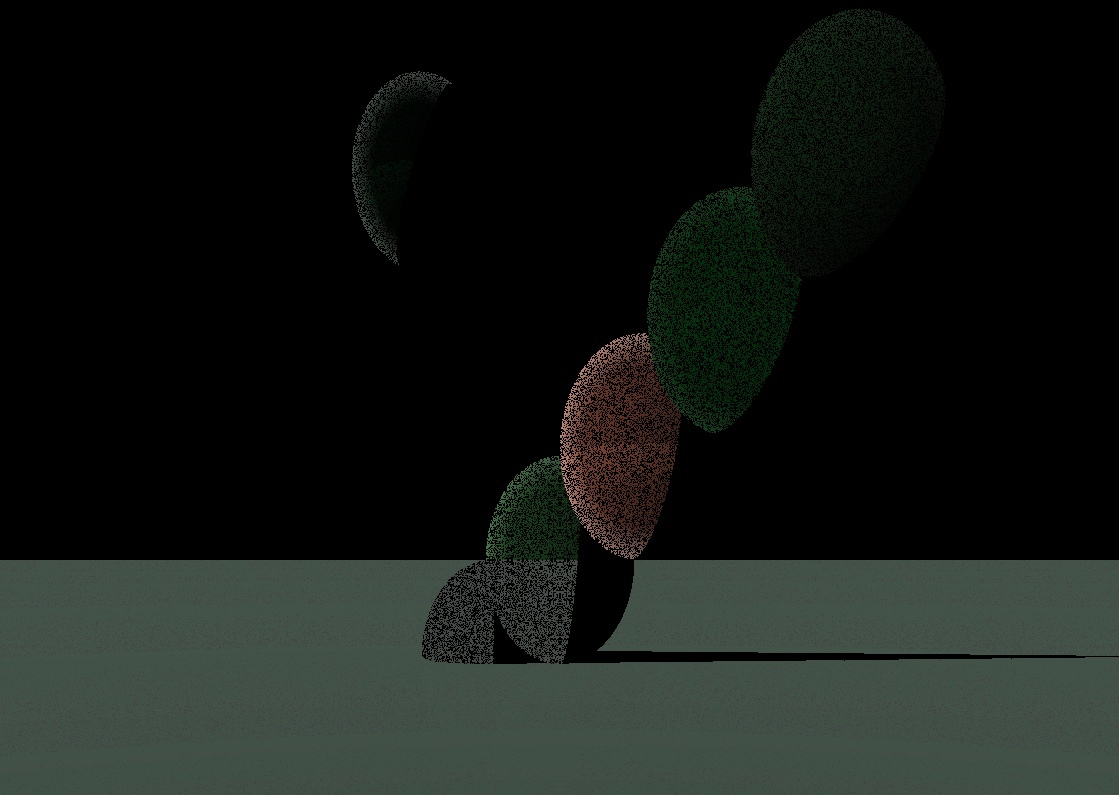
\includegraphics[scale=0.4]{numerous_spheres}
	\caption{Рендер нескольких сфер вместе с плоскостью}
	\label{fig:numerous_spheres}
\end{figure}

\begin{figure}[h]
	\centering
	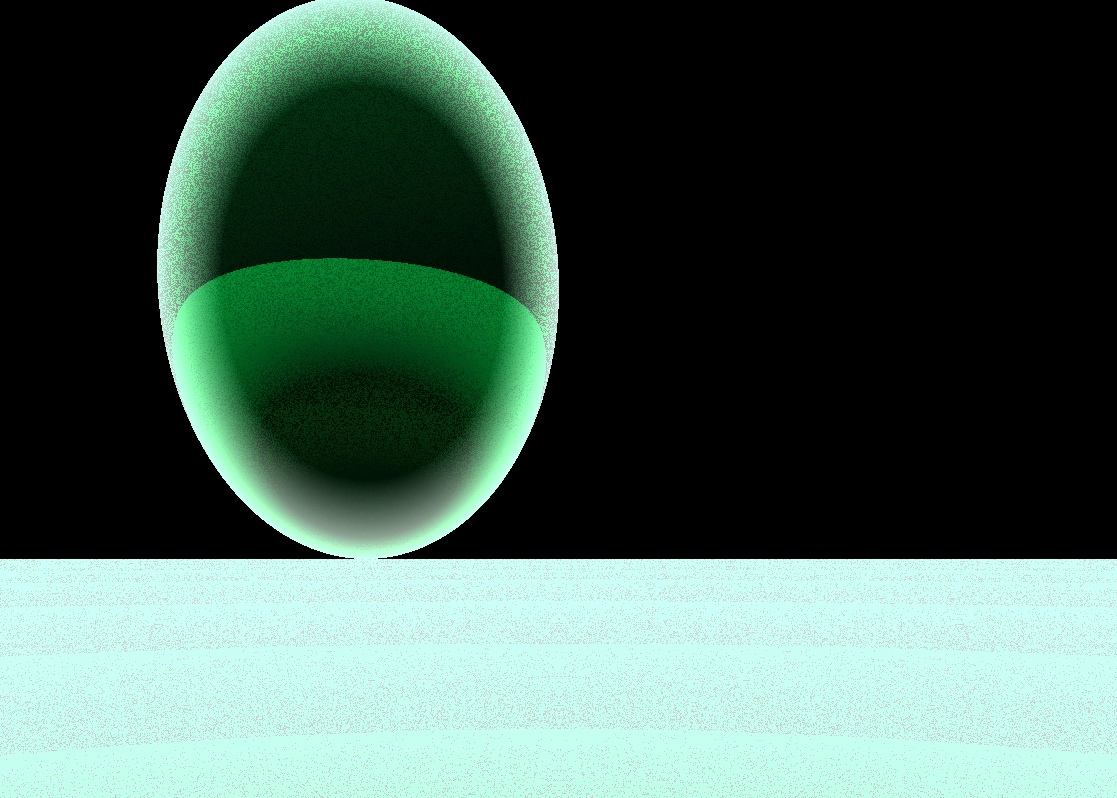
\includegraphics[scale=0.4]{sphere_reflection}
	\caption{Рендер одной сферы с плоскостью}
	\label{fig:numerous_spheres}
\end{figure}